\documentclass[11pt]{article}

\usepackage[a4paper, total={6in, 8in}]{geometry}
\usepackage{geometry}
\usepackage{xcolor}
\usepackage{graphicx}
\usepackage{titling}
\usepackage{afterpage}
\usepackage{fontspec}
\usepackage{titlesec}
\usepackage[bottom]{footmisc}
\usepackage{hyperref}
\usepackage{fancyhdr}

\definecolor{titlepagecolor}{rgb}{0,0,.65}

% Fonts

\setmainfont{IBMPlexSans}[
	Path=./fonts/,
	BoldFont=*-Bold,
	UprightFont=*,
	ItalicFont=*-Italic,
	BoldItalicFont=*-BoldItalic,
]

\newfontfamily{\headerfont}{Serenity}[
	Path=./fonts/,
	UprightFont=*-Medium,
]


% Customization


% Actual document
\geometry{
  a4paper,
  left=2.5cm,
  right=2.5cm,
  top=2.15cm,
  bottom=1.15cm
}
\begin{document}

\setlength\parindent{0pt}
\setlength{\parskip}{.15em}
\pagestyle{empty}

\title{OdenseEmergency in the Cloud \newline}
\author{Alexander Matzen \addvspace{1em} Student Number: 493840 \newline E-mail Address: almat20@student.sdu.dk}
\date{\today}

\begin{titlepage}
\newgeometry{left=3cm,top=3cm, bottom=3cm}
\pagecolor{titlepagecolor}\afterpage{\nopagecolor}
\noindent
\color{white}
\makebox[0pt][l]{\rule{1cm}{2pt}}
\par\addvspace{1cm}
\noindent{\headerfont\Huge{\thetitle}}
\par
{\headerfont\Large{SE05-CCECAA: Cloud Computing and\newline Edge-Cloud Adaptive Architectures}}
\vskip\baselineskip
\noindent
\vfill
\noindent{\theauthor}
\par\addvspace{.5cm}
\noindent{\thedate}
\end{titlepage}


\pagecolor{white}

\tableofcontents
\newpage

\section{Context}
% Show that you understand the context of the use case and its dimensions.

\textit{OdenseEmergency} provides Software-as-a-Service for emergency management to use for both emergency personell and citizens. The company offers their software platform on a global scale and have along with increasing disasters experienced an exponential growth pattern in users.
\newline\newline
The given application is a mobile application that routes people to safe areas in disaster zones and monitors human expression along with location data to encourage users to take the responsible actions and remain calm in difficult situations.

\section{Problem Specification}
% Specify the problems the case addresses.
% Analyze the use case carefully.
% Explain the target requirements (functional and non-functional).

Specified in the case, \textit{OdenseEmergency} has two non-functional requirements: \textbf{performance} and \textbf{energy consumption}. Along with that, the application is considered vital for human lives, and should therefore also provide high \textbf{availability} and \textbf{reliability}.
\newline\newline
Due to the fact, that the application also is used in disasters, we may expect a highly variable rate of active users, so scalability is key to meet the performance requirements.
\newline\newline
Compliance with relevant regulation is also needed, for instance the GDPR, if any European citizen data is stored or processed.

\subsection{Working Questions}
\begin{itemize}
  \item Which Cloud Computing Deployment Model would suit the application best given the requirements?
  \item How can the application be deployed with the minimal energy consumption?
\end{itemize}


\section{Background}
% Here include state-of-the-art knowledge if you want to include some of your academic / tool research.

\subsection{Theory}

\subsubsection{Computing}

The right compute configuration can enable scalability and elasticity, providing a cost benefit but also an availability and performance benefit for the application.
\newline\newline
\textbf{Cloud Computing Models}\footnote{\href{https://engineering.dunelm.com/pizza-as-a-service-2-0-5085cd4c365e}{https://engineering.dunelm.com/pizza-as-a-service-2-0-5085cd4c365e}}\newline
Choosing the right Cloud Computing Model is a decision of defining the responsibility areas between the Cloud Provider and the Cloud Consumer.


\subsubsection{Networking}

A correct networking is necessary for keeping the system reliable and secure, but a good network design can also increase performance for the application.
\newline\newline
\textbf{Virtual Private Cloud} is a private network within the cloud, that can be used to isolate services between cloud ressources. The use of VPCs may be relevant to isolate databases from the public internet, strengthening the database security and reduce latency as the ressources are shared in the network.

\subsection{Toolings}

\textbf{Cloud Architecture Diagram Tool}
To visualize the architecture, I've used the Google Cloud architecture diagramming tool\footnote{\href{https://cloud.google.com/blog/topics/developers-practitioners/introducing-google-cloud-architecture-diagramming-tool}{https://cloud.google.com/blog/topics/developers-practitioners/introducing-google-cloud-architecture-diagramming-tool}}


\textbf{Infrastructure as Code}\newline
In my original plan, I intended to use infrastructure as code for the benefit of version control (Git) and portability. However, due to time management constraints, I was unable to implement this approach.

Infrastructure as code is a good idea because it allows for version control and collaboration using tools like Git. This means that changes to the infrastructure can be tracked, reviewed, and rolled back if necessary. Additionally, infrastructure as code enables portability, allowing for easy migration of the infrastructure to different environments. This can be useful for testing and deployment.

\section{Approach}
% Here you include your architecture as figure(s) and explain your solution, the architecture components, their association, etc. It would be appreciated if you could argue based on what you learned in the lectures/labs, so argue based on network, storage, monitoring, data requirements, and edge-cloud specifications. Do not forget to analyze the use case beforehand.

\subsection{Examination of the App}
I started by examine the application, it consists of two key parts:

\paragraph{Frontend}
A static Progressive Web Application ("PWA") made in React.js, that ships with a multi-stage Dockerfile, containing build and run stages. The build stage simply install NPM dependencies and run "npm run build" and ship the builded application to the run stage. The run stage serves the \textit{build} subdirectory using a regular nginx server.

\paragraph{Backend}
A Node.js Express HTTP Server, that ships with a Dockerfile single stage, installing NPM dependencies and run the server.

\vspace{.25cm}

Both parts uses the HTTP protocol. The backend also uses WebSockets in external communication to the user, and MongoDB Wire Protocol\footnote{\href{https://www.mongodb.com/docs/manual/reference/mongodb-wire-protocol/}{https://www.mongodb.com/docs/manual/reference/mongodb-wire-protocol/}} along with RESP\footnote{\href{https://redis.io/docs/reference/protocol-spec}{https://redis.io/docs/reference/protocol-spec}} system-to-system communication for between the application and respectively MongoDB and Redis.

\subsection{Proposing an architecture}
As the application consists of two parts, I divide them up:

\paragraph{Frontend}
The essential criteria for the frontend application is the delivery of files through the HTTP protocol. To address the sustainability and energy consumption requirements specified by OdenseEmergency, I don't think it's necessary to launch multiple virtual machines (Cloud Compute Engine) across the world just for a high availability nginx server serving static files, neither do I think it's necessary to spin up a container (Cloud Run) or a function (Cloud Functions) for each request to the frontend. Fortunately, Google Cloud provides an Object Storage solution (Cloud Storage), that can be used with a Content Delivery Network (Cloud CDN) to take advantage of the low latency benefit of edge computing and serving files distributed globally. The solution is billed by egress and storage usage, and the compute power (CPU, RAM and IOPS) are shared between Google Cloud Storage customers. Lastly to use Google Cloud CDN and Google Cloud Storage with a custom DNS address and an encrypted connection (TLS (HTTPS)), you must setup a Global HTTP(S) Load Balancer, so this will count in the architecture for the frontend part.

\paragraph{Backend}
The backend has been architectured as a single service, so to prevent any changes to the original application, I would go with running the application as provided. Here I must decide whether I would go for an IaaS, PaaS or FaaS solution, in order to determine this I would look at several key factors:
\begin{enumerate}
	\item Which triggers does the backend service react upon?
	\item How are the Network calls to the backend service from the frontend React application?
	\item How would the application's "popularity" be forecasted scenario-wise?
\end{enumerate}

To address which triggers, the backend service uses, it's only HTTP. The service runs two different types of protocols, an one-way communication protocol (regular HTTP-calls) and a two-way communication protocol (HTTP with WebSockets). As Google Cloud Functions (FaaS) are short-lived function calls, they would fit great for the regular HTTP-calls, but wouldn't fit that great for WebSockets as they rely on long-lived connections to the server. Therefore an IaaS or PaaS solution would fit better for this factor.

The React app (frontend) has multiple calls to the backend in a short timespan, that could imply a per-resource-usage pricing model would better than per-request pricing model.

Last, the application's popularity I would describe as heavily spike-dependent, as hopefully the application is not used that often, but should be able to scale indefinitely, hence why a hyper-scaling solution like Kubernetes (GKE Standard or GKE Autopilot), Google Cloud Run or Google Cloud Functions.


\

\section{Implementation}
% Explain how you implement the app locally, then deploy it on GCP, and how the adaptation system (if any) may work. Explain the technologies you use for the non-functional requirements testing.


\section{Evaluation}
% Here include a report of your test results and discuss their validity and alignment with objectives.

To test the implementation properly, an 

\begin{figure}[h]
	\centering
	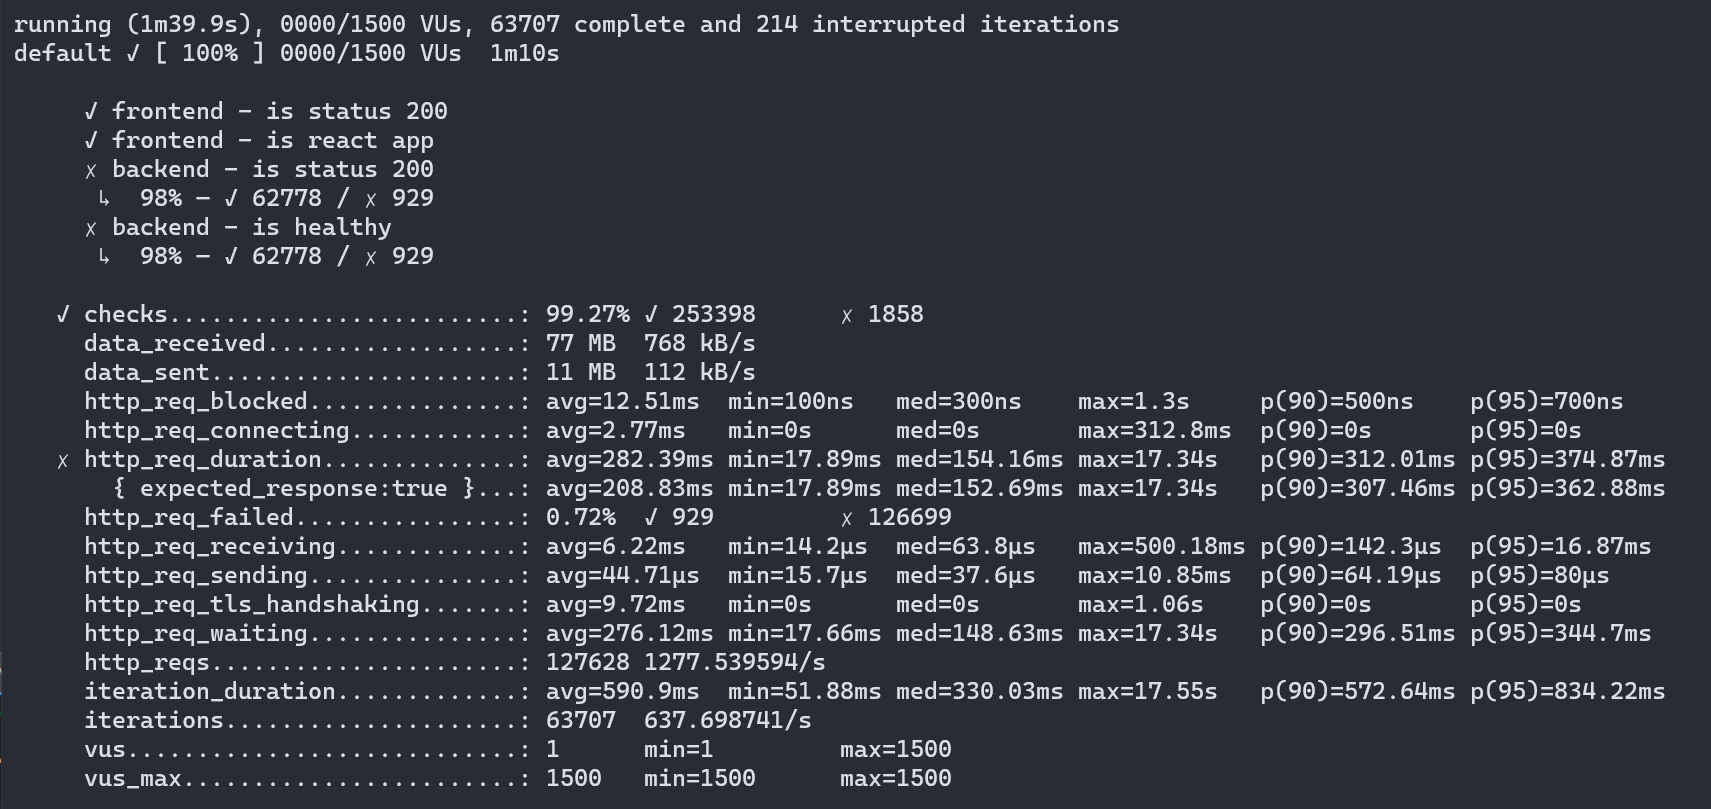
\includegraphics[width=0.7\linewidth]{scr_k6_loadtest}
	\caption{Screenshot of K6 Load Test Result}
	\label{fig:scr:k6:loadtest}
\end{figure}

As shown in Figure \ref{fig:scr:k6:loadtest}, the frontend was able to pass the checks criteria, meanwhile the backend was not. The backend uses Google Cloud Run, which scales containers, and without having 

\section{Discussion}
% Final discussions and lessons learned and how your suggested architecture could be re-used.




\end{document}
